\documentclass{beamer}
\usepackage{graphicx}
\usepackage{amssymb,amsfonts,amsmath}
% \usepackage{tikz,tkz-euclide}
\usepackage{subcaption}
\usepackage{xcolor}
% \usepackage{parskip}
% \usetikzlibrary{arrows.meta}
% \usetikzlibrary{calc,patterns}
\usefonttheme[onlymath]{serif}
% \usetheme{Berlin}
\title{Weekly Report}
\author{WU Zihan}
\begin{document}
\maketitle
% \begin{frame}
%     \frametitle{Outline}
%     \tableofcontents
% \end{frame}

\section{Results}
\begin{frame}
    \frametitle{Results for simulated data matrix}
    \begin{columns}[T]
        \begin{column}{0.5\textwidth}
            \centering
            \textbf{Experiment settings}
            % A_{MxN}, M = N = 2000
            % 15 biclusters preset
            % Each bicluster has random height and width from 50 to 200
            % noise level = 1% of the maximum value
            \begin{itemize}
                \item $A_{M\times N}$, $M = N = 2000$
                \item Biclusters number $k = 15$
                \item Bicluster height $m_i$ and width $n_i$ subject to uniform distribution $U(50, 200)$
                \item Noise level $\sigma_{\text{Noise}} = 10^{-5} \times \max(A)$
            \end{itemize}
            \textbf{Experiment results}
    \textcolor{red}{$100\%$ on both precision and recall}
        \end{column}
        \begin{column}{0.5\textwidth}
            \vspace{-1cm}
            \centering
            
            \begin{figure}[htb]
                \centering
                \begin{subfigure}[b]{\textwidth}
                    \centering
                    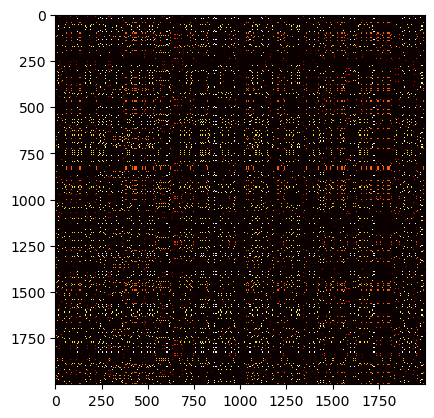
\includegraphics[width=0.6\linewidth]{image1.png}
                    \caption{Ground truth}
                    \label{fig:image1}
                \end{subfigure}
                % \vspace{-0.5cm}
                \begin{subfigure}[b]{\textwidth}
                    \centering
                    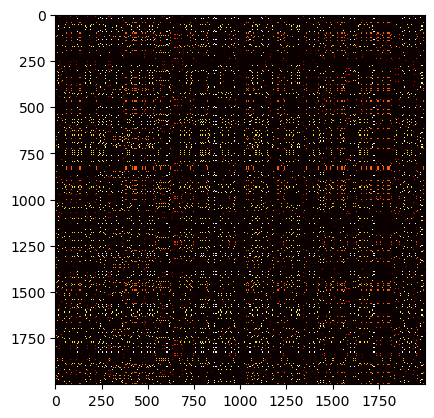
\includegraphics[width=0.6\linewidth]{image2.png}
                    \caption{Biclusters detected}
                    \label{fig:image2}
                \end{subfigure}
                \vspace{-0.8cm}
                \caption{Comparison of ground truth and detected biclusters}
                \label{fig:comparison}
            \end{figure}
        \end{column}
    \end{columns}
\end{frame}

\section{Methods}
\begin{frame}
    \frametitle{Methods}

    \begin{columns}
        \begin{column}{0.5\textwidth}
            \centering
            \textbf{Score Function for Biclustering}
            \begin{itemize}
                \item $$\langle x, y \rangle = \exp(-\frac{||x - y||_1^2}{2\alpha||x||_1||y||_1})$$
                \item Use the inner product above to substitute for the co-variance
            \end{itemize}
        \end{column}
        \begin{column}{0.5\textwidth}
            \centering
            \textbf{Selection of $S_{\text{th}}$}
            \begin{itemize}
                \item For a bicluster $B \in \mathbb{R}^{T_m \times T_n}$
                \item Suppose $\max(||B||_1,||B^{\top}||_1) \le B_{\max}$
                \item If $B$ is a bicluster with $\beta = 1\%$ tolerance, then
                \item Denot $\min (T_m, T_n) = t$, then
                \begin{align*}
                    S &\le \frac{1-\exp ^{-\frac{1}{2\alpha t ^2}}}{t - 1} \\
                    &\le \frac{1}{2 \alpha t ^2(t - 1)}
                \end{align*}
                \item In the experiment, $\alpha = 0.01, S_{\text{th}} = 0.02$
            \end{itemize}
        \end{column}
    \end{columns}

\end{frame}


\end{document}